\chapter{Правила использования шаблона}\label{app-manual}

Настоящий шаблон все еще несколько несовершенен в плане оформления: например, неправильная нумерация приложений, и еще несколько нюансов. В последующих версиях это будет исправляться.

Ниже описана структура исходных текстов шаблона (и, соответственно, структура исходных текстов ПЗ).

Головной файл --- \texttt{thesis-template.tex}. Его задача --- <<склеить>> вместе разные части ПЗ. Каждая часть (реферат, введение, каждая содержательная глава, заключение, библиография, приложения) выделяется в отдельный файл. 

\begin{itemize}
	\item[] \texttt{thesis-macro.tex} --- содержит определения различных макрокоманд, которые часто используются в конкретной работе, например, определения окружения для теорем, некоторые часто используемые формулы, и т.п.;
	\item[] \texttt{thesis-abstract.tex} --- содержит аннотацию;
	\item[] \texttt{thesis-intro.tex} --- содержит введение;
	\item[] \texttt{thesis-chapter1.tex} --- текст первой главы;
	\item[] \texttt{thesis-chapter2.tex} --- текст второй главы;
	\item[] \texttt{thesis-chapter3.tex} --- текст третьей главы;
	\item[] \texttt{thesis-bibl.tex} --- список литературы (только подключение к
	проекту);
	\item[] \texttt{biblio.bib} --- собственно библиография (в формате BibTeX);
	\item[] \texttt{thesis-conclusion.tex} --- заключение;
	\item[] \texttt{thesis-appendix1.tex} --- первое приложение;
	\item[] \texttt{thesis-appendix2.tex} --- второе приложение;
\end{itemize}


%Одна из первых вещей, которые необходимо сделать при использовании данного шаблона --- это отредактировать аргумент команды \verb|\headertext| в начале головного файла.

Головной файл нужно менять лишь тогда, когда нужно добавить в проект новый файл, или удалить существующий (см. команду \verb|\input|). Обычно, это требуется, когда нужно добавить/удалить приложения.

Для того, чтобы \LaTeX{} при компиляции автоматически <<подхватил>> задание, его нужно сохранить в формате pdf (например, с помощью вирутального принтера), поместить в ту же папку \texttt{/title} и назвать \texttt{task.pdf}. Точно также следует поступить с титульной страницей (\texttt{title.pdf}). При оформлении ПЗ для ВКР следует дополнительно поместить в папку \texttt{/title} pdf-версию листа с подписями, назвав файл \texttt{title-dep22.pdf}. После этого, нужно раскомментировать команду \verb|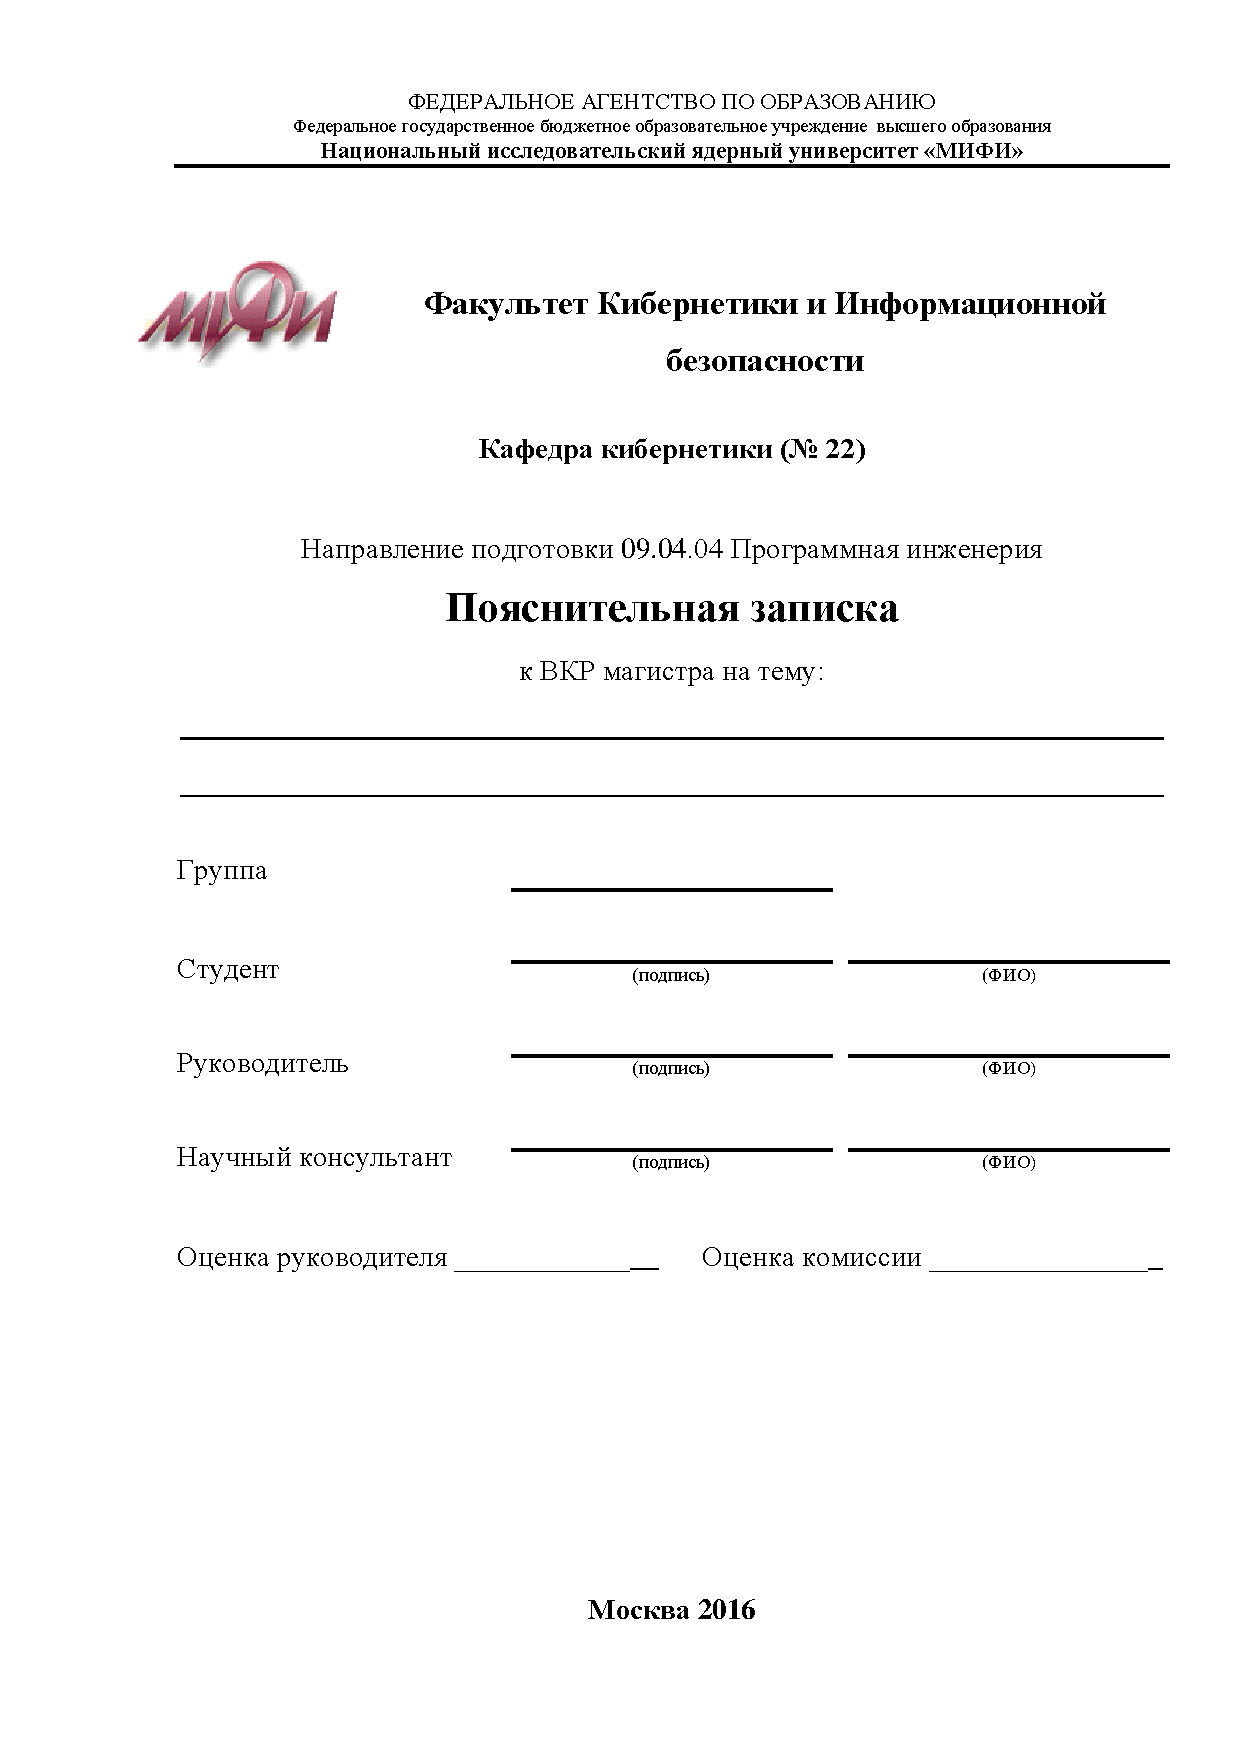
\includepdf[pages={-}, offset=0mm -0mm]{title/title-dep22.pdf}| в начале головного файла. Образцы и Word-шаблоны титульных листов для (РС)ПЗ к УИРам, НИРам, практикам и ВКР лежат в папках \texttt{/title/магистры} и \texttt{/title/бакалавры}.

В этой версии шаблона используется BibTeX, поэтому для оформления списка
литературы используются два файла: \texttt{thesis-bibl.tex} и
\texttt{biblio.bib}. Использование BibTex дает ряд преимуществ. Не нужно
заботиться о порядке сортировки, это делается автоматически; не нужно заботиться,
на какие элементы библиографии есть ссылки --- печатаются только использованные в
тексте элементы. Кроме того, многие курсовые проекты выполняются на протяжении ряда лет. С BibTex проще собирать список литературы и управлять им.

\textbf{Замечание}. В шаблоне используется пакет \texttt{hyperref}, который делает две вещи: все перекрестные ссылки <<кликабельны>>, а также выделены (красной) рамочкой. Эти рамки \textit{не выводятся на печать}. Вместо цветных рамок, возможны другие способы выделения ссылок (см. документацию пакета).
